\documentclass[12pt]{report}
\usepackage[utf8]{inputenc}
\usepackage[french]{babel}
\usepackage[T1]{fontenc}
\usepackage{amsmath}
\usepackage{amsfonts}
\usepackage{amssymb}
\usepackage{graphicx}
\usepackage{titlesec}
\usepackage{caption}
\usepackage{titling}
\usepackage{booktabs}
\usepackage{enumitem}
\usepackage{eurosym}
\usepackage{epigraph}
\usepackage{hyperref}
\usepackage{fontspec}
\usepackage{ragged2e}
\usepackage{parskip}
\usepackage{wrapfig}
\usepackage{calc}
\usepackage{float}

\graphicspath{ {img/} }
\setlength{\droptitle}{-10em}
\titleformat{\chapter}[hang]{\normalfont\huge\bfseries}{\thechapter. }{0em}{}

\begin{document}

\title{
	{\Huge Projet OCR}\\
	\vspace{2em}
	{\Huge Rapport de soutenance}\\
	{\large Wizard Neurons}
}
\author{
	Antoine Gonzalez\\
	Cédric Parpet
	\and
	Louis Le-Gatt\\
	Jeremy Salfati}
\date{
	\vspace{15em}
	{Dossier Projet Informatique\\
	Info-Spé EPITA\\
	Octobre 2018}
}

\maketitle
\tableofcontents

\chapter{Introduction}

Cette première moitié de projet aura été assez difficile, mais très intéressante. N'ayant eu que peu de cours de C, il nous a fallu apprendre par nous même tout ce dont nous avions besoin. De plus, ce projet nous laisse bien moins de libertés que celui du semestre précédent, plus de limites nous sont imposées, tant sur le projet lui-même que sur la manière de l'implémenter. Ce qui nous force à chercher des solutions parfois moins évidentes.

Cependant, le groupe est motivé: un OCR est très intéressant à mettre en place et nous permet de nous essayer à beaucoup de concepts différents de la programmation: l'interface utilisateur avec GTK, le traitement d'image avec la SDL, et enfin l'intelligence artificielle (buzzword du moment) avec les réseaux de neuronnes. Et surtout, le langage C qui nous a été imposé est un classique de la programmation, et apprendre à l'utiliser nous permettra de mieux saisir certains concepts de la programmation avec deslangages plus haut-niveaux, et de comprendre par exemple la gestion de la mémoire.

C'est donc avec soif de connaissances que nous nous sommes mis au travail, en quête du meilleur OCR réalisable. Durant ces premières semaines, chacun a pu expérimenter avec sa partie. Nous possédons désormais les connaissances et outils nécéssaires à la bonne réalisation du projet.

Dans ce rapport, nous allons présenter notre vision du projet ainsi que les avancées que nous avons réalisé, les difficultés rencontrées, et enfin nos plans pour la seconde soutenance.

\begin{figure}
    \centering
    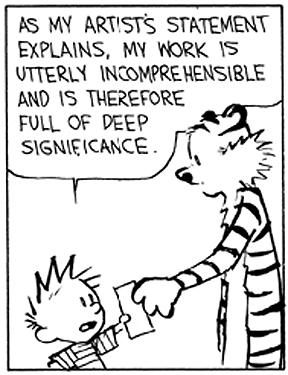
\includegraphics[width=0.6\textwidth]{project_mood_S1}
    \caption*{\textit{Calvin and Hobbes}, Bill Watterson}
\end{figure}

\chapter{Répartition des tâches}

Afin de rester organisés tout au long de ce projet, nous nous sommes réparties les tâches de la manière suivante.

\begin{center}
    \begin{tabular}{@{} l *4c @{}}
        \toprule
        \multicolumn{1}{c}{}    & \textbf{Antoine}  & \textbf{Louis}  & \textbf{Cédric} & \textbf{Jeremy} \\ 
        \midrule
        Chargement de l'image & & & & X \\
        Traitement de l'image & & X & & \\
        Découpage de l'image & & & X & \\
        Réseau Neuronal & X & & & \\
        Sauvegarde des résultats & & & & X \\
        Interface Utilisateur & & & & X \\
        \bottomrule
    \end{tabular}
\end{center}


En somme, Antoine s'occupera de tout ce qui touchera de près ou de loin au réseau de neuronnes. Louis se chargera du traitement primaire de l'images (black\&white ou grayscale, création d'une toolbox pour la manipulation des pixels...). Cédric devra s'occuper du découpage de l'image en lignes puis caractères, et de la reconstruction du texte reconnu par le réseau de neuronnes. Enfin, Jeremy sera en charge de l'interface utilisateur, afin de pouvoir utiliser tous nos systèmes de manière intuitive.

Bien entendu, chaque membre reste disponible pour aider les autres en fonction des besoins et du temps disponible.

\chapter{Diagramme Fonctionnel de l'OCR}

Afin que chaque membre comprenne parfaitement ce qui est attendu de sa partie et comment elle devra interagir avec celle des autres membres, nous avons réalisé un diagramme fonctionnel de l'OCR. On peut y voir le déroulement de son éxecution, du moment où l'utilisateur charge une image, au moment où le texte détecté est affiché et enrgistré \textit{(voir figure ci-dessous)}.

Comme on peut le voir, chaque partie interagit de manière simple avec le reste, et possède un but bien définit. Chaque morceau de l'OCR n'appelle qu'une unique autre partie, ce qui limite les erreurs potentielles d'appels croisés entre les multiples fonctions. Chaque membre du groupe n'a donc qu'à penser à une seule autre partie. Il lui suffit de spécifier quel type de valeur il attend en retour, et quel type de valeur il est capable d'envoyer. La partie suivante n'a qu'à s'adapter à ces règles, et faire de même.

\begin{figure}[H]
    \centering
    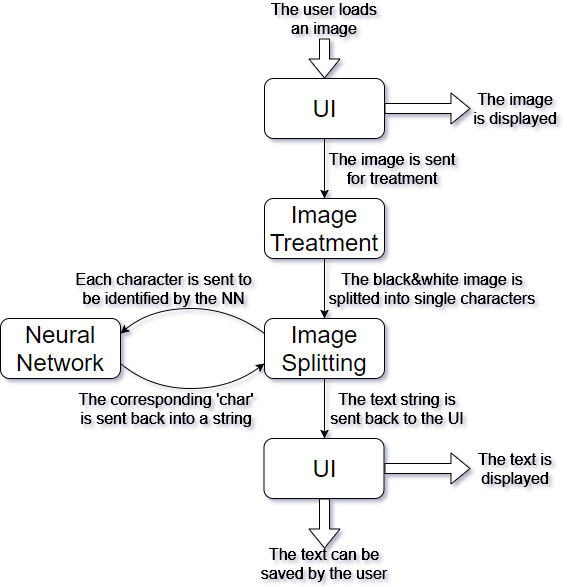
\includegraphics[width=1\textwidth]{OCR_functionnal_diagram}
    \caption{Functional diagram}
\end{figure}

\chapter{Avancement}

\section{Traitement de l'image (Louis)}

...

\section{Découpage de l'image (Cédric)}

...

%\begin{itemize}[label=\textbullet]
%	\item Le joueur \textit{player\_A} déplace une unité (numéroté 3) de la case $(5;3)$ vers la $(5;5)$
%	\item Le client envoie le message\textit{ “CMOV|3\#5.3\#5.5”}
%	\item Le serveur reçoit et renvoie aux clients\textit{ “SMOV|player\_A\#3\#5.3\#5.5”}
%	\item Les clients reçoivent le message et le décryptent pour déplacer l’unité du \textit{playerF\_A}
%\end{itemize}

\section{Réseau neuronal (Antoine)}

Pour le réseau de neurones capable d'apprendre la porte logique XOR, je suis partit d'un design classique: 2 entrées, 1 couche cachée contenant 2 neurones, 1 sortie, et 1 biais entre chaque couche. Afin que les données soient organisées, j'ai opté pour des tableaux pour stocker le contenu des noeuds et les poids (les poids entre l'entrée et le \textit{hidden layer} sont nécéssairement stockés dans une matrice). 

La fonction d'activation que j'ai choisi est la fonction sigmoïde, suffisante pour un réseau de neuronne de cette taille. Tout cela me donne un réseau qui prend cette forme:

\begin{figure}[H]
    \centering
    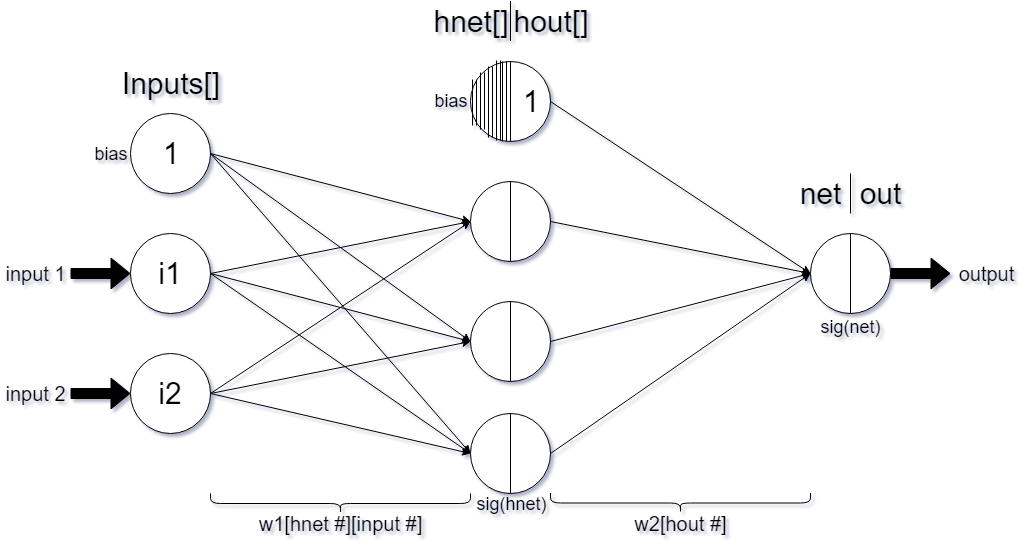
\includegraphics[width=1\textwidth]{XOR_Neural_Network}
    \caption{XOR neural network}
\end{figure}

Mais il ne s'agit ici que du XOR, un \textit{proof of concept}. Pour le véritable réseau de neuronnes, il faudra traiter des caractères sous forme d'images de dimensions 28x28 pixels, soit 784 entrées. Il me faudra expérimenter avec le \textit{hidden layer} afin de trouver combien de neuronnes seront nécéssaires, voire s'il est utile d'ajouter une couche supplémentaire. Enfin, pour la sortie, nous allons nous contenter de la reconnaissance des chiffres et des lettres (majuscules et minuscules), soit 62 caractères, donc 62 sorties.

Afin d'entrainer cette future intelligence artificielle, je compte pour le moment utiliser les ressources fournies par NIST dans son \textit{NIST Special Database 19}, disponible à l'adresse suivante: \url{https://catalog.data.gov/dataset/nist-handprinted-forms-and-characters-nist-special-database-19}. 

Je pense qu'une des difficultés principales de la deuxième partie du projet sera d'apprendre à utiliser ces données (en extraire les images et les valeurs attendues), mais cette archive est très complète et contient suffisament d'exemples pour entraîner le réseau de neuronnes.

\section{Interface utilisateur (Jeremy)}

...

\newpage
\chapter{Avances, retards, difficultés rencontrées}

\section*{Traitement de l'image}

...

\section*{Découpage de l'image}

...

\section*{Réseau neuronal}

Comme dit plus haut, j'ai eu beaucoup de difficultés à comprendre pourquoi le réseau de neuronnes, qui la majorité du temps fonctionne sans problème, n'apprenait parfois pas la moitié de la table de vérité du XOR. Il s'agissait en fait d'un problème de minimum local. N'ayant pas réussi à implémenter de momentum, je me suis contenté de mitiger la probabilité de tomber dans un minimum local en ajoutant un neurone supplémentaire dans la couche cachée.

Pour le réseau de neurone de l'OCR, j'utiliserai simplement un seed prédéfinit pour le random: une valeur d'initialisation de l'aléatoire pour laquelle l'apprentissage fonctionne, car il n'est pas nécéssaire d'avoir un aléatoire différent à chaque apprentissage du réseau, du moment que celui-ci fonctionne.

A cause de ce problème sur lequel j'ai passé trop de temps, je n'ai pas pu commencer à m'occuper de l'enregistrement des poids du réseau neuronal. Il faudra donc mettre cela en place pour la soutenance finale.

Autrement, l'autre difficulté de cette partie a été d'apprendre à utiliser les pointeurs et \textit malloc pour utiliser les tableaux en C.

\section*{Interface utilisateur}

...

\chapter{À venir}

\begin{itemize}
	\item \textbf{Traitement :} corriger ou adapter le traitement en fonction des besoins après des tests sur le réseau de neuronnes réel.
	\item \textbf{Découpage :} reconstruction du texte. Normalement, l'implémentation récursive permettra une reconstruction simple.
	\item \textbf{Réseau neuronal :} véritable réseau de neuronnes de l'OCR, sauvegarde des poids.
	\item \textbf{Interface :} lier l'interface aux différentes fonctions.
\end{itemize}

\chapter{Expériences personnelles}

\begin{itemize}
	\item \textbf{Louis :} <=5 lignes
	\item \textbf{Cédric :} <=5 lignes
	\item \textbf{Antoine :} Cette première partie du projet a été très intéressante pour moi. Cela m'a permis d'apprendre ce qu'est un réseau neuronal, comment cela fonctionne, et comment en créer un. L'intelligence artificielle n'est plus un concept totalement opaque pour moi, et je comprend désormais ce dont il s'agit. Après avoir traité de simples 0 et 1 pour une porte logique, j'ai hate de créer le réseau qui sera capable de traiter des images de caractères, bien que cela sera difficile à mettre en place.
	\item \textbf{Jeremy :} <=5 lignes
\end{itemize}

\chapter{Conclusion}

La première soutenance de projet arrive, et le groupe est satisfait de son travail. Notre réseau de neuronne XOR fonctionne, nous disposons désormais d'outils de traitement d'image qui faciliteront notre travail à venir, le découpage de l'image en lignes puis caractères fonctionne parfaitement, et l'interface utilisateur avance bien. Toutefois, il reste beaucoup de travail, et le plus difficile reste à venir. Le réseau de neurones attendu est beaucoup plus complexe que celui chargé d'apprendre la porte logique XOR, et il faut également l'entrainer. L'interface doit être terminée et reliée aux fonctions de l'OCR au plus vite. Et il faudra probablement corriger l'implémentation du traitement d'images et du découpage en fonction des résultats de futurs tests "en conditions réelles".

Malgré les difficultés rencontrées, le groupe est motivé, et très confiant. Bien que certaines parties vont devenir plus chargées, d'autres vont s'alléger, permettant ainsi aux membres d'aider les autres plus facilement. L'OCR sera donc réalisé dans son entièreté en temps et en heure.

\vfill

%\begin{figure}[H]
%    \centering
%    \includegraphics[width=0.8\textwidth]{project_real_mood}
%\end{figure}

\end{document}
